% flashcards-title: Addition split into tens and ones on a whole-number line
% flashcards-desc: A line starts at thirty-eight, jumps right by twenty to fifty-eight, then right by four to an unknown endpoint.
\documentclass[dvisvgm,tikz,border=8pt]{standalone}
\usetikzlibrary{arrows.meta,patterns}

\definecolor{qraNavy}{HTML}{17324D}
\definecolor{qraBlue}{HTML}{2B6CB0}
\definecolor{qraGold}{HTML}{B7791F}
\definecolor{qraPale}{HTML}{EAF2F8}
\definecolor{qraGray}{HTML}{5C6773}

\tikzset{
  qra axis/.style={draw=qraNavy, line width=1.2pt},
  qra tick/.style={draw=qraNavy, line width=1pt},
  qra guide/.style={draw=qraGray, densely dashed, line width=0.8pt},
  qra counter/.style={circle, draw=qraNavy, fill=qraPale, line width=0.9pt, minimum size=7mm, inner sep=0pt},
  qra label/.style={font=\sffamily\bfseries, text=qraNavy},
  qra small label/.style={font=\sffamily, text=qraNavy},
}

\begin{document}
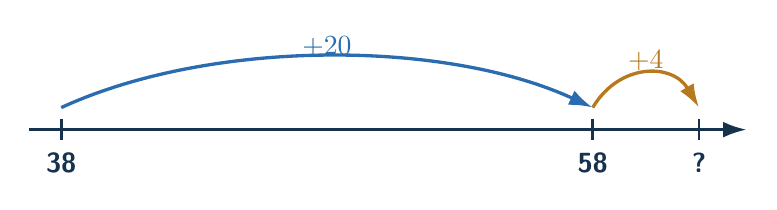
\begin{tikzpicture}[x=1.35cm,y=1cm]
  \draw[qra axis, -{Latex[length=3mm,width=2mm]}] (-0.3,0) -- (6.45,0);
  \foreach \x/\lab in {0/38,5/58,6/?} {
    \draw[qra tick] (\x,-0.13) -- (\x,0.13);
    \node[qra label, below=5pt] at (\x,0) {\lab};
  }
  \draw[qra axis, qraBlue, -{Latex[length=3mm,width=2mm]}] (0,0.28) .. controls (1.4,1.15) and (3.6,1.15) .. (5,0.28);
  \node[qra label, text=qraBlue] at (2.5,1.05) {$+20$};
  \draw[qra axis, qraGold, -{Latex[length=3mm,width=2mm]}] (5,0.28) .. controls (5.25,0.85) and (5.75,0.85) .. (6,0.28);
  \node[qra label, text=qraGold] at (5.5,0.88) {$+4$};
\end{tikzpicture}
\end{document}
